% Options for packages loaded elsewhere
\PassOptionsToPackage{unicode}{hyperref}
\PassOptionsToPackage{hyphens}{url}
\PassOptionsToPackage{dvipsnames,svgnames,x11names}{xcolor}
%
\documentclass[
  letterpaper,
  DIV=11,
  numbers=noendperiod]{scrartcl}

\usepackage{amsmath,amssymb}
\usepackage{iftex}
\ifPDFTeX
  \usepackage[T1]{fontenc}
  \usepackage[utf8]{inputenc}
  \usepackage{textcomp} % provide euro and other symbols
\else % if luatex or xetex
  \usepackage{unicode-math}
  \defaultfontfeatures{Scale=MatchLowercase}
  \defaultfontfeatures[\rmfamily]{Ligatures=TeX,Scale=1}
\fi
\usepackage{lmodern}
\ifPDFTeX\else  
    % xetex/luatex font selection
\fi
% Use upquote if available, for straight quotes in verbatim environments
\IfFileExists{upquote.sty}{\usepackage{upquote}}{}
\IfFileExists{microtype.sty}{% use microtype if available
  \usepackage[]{microtype}
  \UseMicrotypeSet[protrusion]{basicmath} % disable protrusion for tt fonts
}{}
\makeatletter
\@ifundefined{KOMAClassName}{% if non-KOMA class
  \IfFileExists{parskip.sty}{%
    \usepackage{parskip}
  }{% else
    \setlength{\parindent}{0pt}
    \setlength{\parskip}{6pt plus 2pt minus 1pt}}
}{% if KOMA class
  \KOMAoptions{parskip=half}}
\makeatother
\usepackage{xcolor}
\setlength{\emergencystretch}{3em} % prevent overfull lines
\setcounter{secnumdepth}{-\maxdimen} % remove section numbering
% Make \paragraph and \subparagraph free-standing
\ifx\paragraph\undefined\else
  \let\oldparagraph\paragraph
  \renewcommand{\paragraph}[1]{\oldparagraph{#1}\mbox{}}
\fi
\ifx\subparagraph\undefined\else
  \let\oldsubparagraph\subparagraph
  \renewcommand{\subparagraph}[1]{\oldsubparagraph{#1}\mbox{}}
\fi

\usepackage{color}
\usepackage{fancyvrb}
\newcommand{\VerbBar}{|}
\newcommand{\VERB}{\Verb[commandchars=\\\{\}]}
\DefineVerbatimEnvironment{Highlighting}{Verbatim}{commandchars=\\\{\}}
% Add ',fontsize=\small' for more characters per line
\usepackage{framed}
\definecolor{shadecolor}{RGB}{241,243,245}
\newenvironment{Shaded}{\begin{snugshade}}{\end{snugshade}}
\newcommand{\AlertTok}[1]{\textcolor[rgb]{0.68,0.00,0.00}{#1}}
\newcommand{\AnnotationTok}[1]{\textcolor[rgb]{0.37,0.37,0.37}{#1}}
\newcommand{\AttributeTok}[1]{\textcolor[rgb]{0.40,0.45,0.13}{#1}}
\newcommand{\BaseNTok}[1]{\textcolor[rgb]{0.68,0.00,0.00}{#1}}
\newcommand{\BuiltInTok}[1]{\textcolor[rgb]{0.00,0.23,0.31}{#1}}
\newcommand{\CharTok}[1]{\textcolor[rgb]{0.13,0.47,0.30}{#1}}
\newcommand{\CommentTok}[1]{\textcolor[rgb]{0.37,0.37,0.37}{#1}}
\newcommand{\CommentVarTok}[1]{\textcolor[rgb]{0.37,0.37,0.37}{\textit{#1}}}
\newcommand{\ConstantTok}[1]{\textcolor[rgb]{0.56,0.35,0.01}{#1}}
\newcommand{\ControlFlowTok}[1]{\textcolor[rgb]{0.00,0.23,0.31}{#1}}
\newcommand{\DataTypeTok}[1]{\textcolor[rgb]{0.68,0.00,0.00}{#1}}
\newcommand{\DecValTok}[1]{\textcolor[rgb]{0.68,0.00,0.00}{#1}}
\newcommand{\DocumentationTok}[1]{\textcolor[rgb]{0.37,0.37,0.37}{\textit{#1}}}
\newcommand{\ErrorTok}[1]{\textcolor[rgb]{0.68,0.00,0.00}{#1}}
\newcommand{\ExtensionTok}[1]{\textcolor[rgb]{0.00,0.23,0.31}{#1}}
\newcommand{\FloatTok}[1]{\textcolor[rgb]{0.68,0.00,0.00}{#1}}
\newcommand{\FunctionTok}[1]{\textcolor[rgb]{0.28,0.35,0.67}{#1}}
\newcommand{\ImportTok}[1]{\textcolor[rgb]{0.00,0.46,0.62}{#1}}
\newcommand{\InformationTok}[1]{\textcolor[rgb]{0.37,0.37,0.37}{#1}}
\newcommand{\KeywordTok}[1]{\textcolor[rgb]{0.00,0.23,0.31}{#1}}
\newcommand{\NormalTok}[1]{\textcolor[rgb]{0.00,0.23,0.31}{#1}}
\newcommand{\OperatorTok}[1]{\textcolor[rgb]{0.37,0.37,0.37}{#1}}
\newcommand{\OtherTok}[1]{\textcolor[rgb]{0.00,0.23,0.31}{#1}}
\newcommand{\PreprocessorTok}[1]{\textcolor[rgb]{0.68,0.00,0.00}{#1}}
\newcommand{\RegionMarkerTok}[1]{\textcolor[rgb]{0.00,0.23,0.31}{#1}}
\newcommand{\SpecialCharTok}[1]{\textcolor[rgb]{0.37,0.37,0.37}{#1}}
\newcommand{\SpecialStringTok}[1]{\textcolor[rgb]{0.13,0.47,0.30}{#1}}
\newcommand{\StringTok}[1]{\textcolor[rgb]{0.13,0.47,0.30}{#1}}
\newcommand{\VariableTok}[1]{\textcolor[rgb]{0.07,0.07,0.07}{#1}}
\newcommand{\VerbatimStringTok}[1]{\textcolor[rgb]{0.13,0.47,0.30}{#1}}
\newcommand{\WarningTok}[1]{\textcolor[rgb]{0.37,0.37,0.37}{\textit{#1}}}

\providecommand{\tightlist}{%
  \setlength{\itemsep}{0pt}\setlength{\parskip}{0pt}}\usepackage{longtable,booktabs,array}
\usepackage{calc} % for calculating minipage widths
% Correct order of tables after \paragraph or \subparagraph
\usepackage{etoolbox}
\makeatletter
\patchcmd\longtable{\par}{\if@noskipsec\mbox{}\fi\par}{}{}
\makeatother
% Allow footnotes in longtable head/foot
\IfFileExists{footnotehyper.sty}{\usepackage{footnotehyper}}{\usepackage{footnote}}
\makesavenoteenv{longtable}
\usepackage{graphicx}
\makeatletter
\def\maxwidth{\ifdim\Gin@nat@width>\linewidth\linewidth\else\Gin@nat@width\fi}
\def\maxheight{\ifdim\Gin@nat@height>\textheight\textheight\else\Gin@nat@height\fi}
\makeatother
% Scale images if necessary, so that they will not overflow the page
% margins by default, and it is still possible to overwrite the defaults
% using explicit options in \includegraphics[width, height, ...]{}
\setkeys{Gin}{width=\maxwidth,height=\maxheight,keepaspectratio}
% Set default figure placement to htbp
\makeatletter
\def\fps@figure{htbp}
\makeatother
\newlength{\cslhangindent}
\setlength{\cslhangindent}{1.5em}
\newlength{\csllabelwidth}
\setlength{\csllabelwidth}{3em}
\newlength{\cslentryspacingunit} % times entry-spacing
\setlength{\cslentryspacingunit}{\parskip}
\newenvironment{CSLReferences}[2] % #1 hanging-ident, #2 entry spacing
 {% don't indent paragraphs
  \setlength{\parindent}{0pt}
  % turn on hanging indent if param 1 is 1
  \ifodd #1
  \let\oldpar\par
  \def\par{\hangindent=\cslhangindent\oldpar}
  \fi
  % set entry spacing
  \setlength{\parskip}{#2\cslentryspacingunit}
 }%
 {}
\usepackage{calc}
\newcommand{\CSLBlock}[1]{#1\hfill\break}
\newcommand{\CSLLeftMargin}[1]{\parbox[t]{\csllabelwidth}{#1}}
\newcommand{\CSLRightInline}[1]{\parbox[t]{\linewidth - \csllabelwidth}{#1}\break}
\newcommand{\CSLIndent}[1]{\hspace{\cslhangindent}#1}

\usepackage{booktabs}
\usepackage{longtable}
\usepackage{array}
\usepackage{multirow}
\usepackage{wrapfig}
\usepackage{float}
\usepackage{colortbl}
\usepackage{pdflscape}
\usepackage{tabu}
\usepackage{threeparttable}
\usepackage{threeparttablex}
\usepackage[normalem]{ulem}
\usepackage{makecell}
\usepackage{xcolor}
\KOMAoption{captions}{tableheading}
\makeatletter
\makeatother
\makeatletter
\makeatother
\makeatletter
\@ifpackageloaded{caption}{}{\usepackage{caption}}
\AtBeginDocument{%
\ifdefined\contentsname
  \renewcommand*\contentsname{Table of contents}
\else
  \newcommand\contentsname{Table of contents}
\fi
\ifdefined\listfigurename
  \renewcommand*\listfigurename{List of Figures}
\else
  \newcommand\listfigurename{List of Figures}
\fi
\ifdefined\listtablename
  \renewcommand*\listtablename{List of Tables}
\else
  \newcommand\listtablename{List of Tables}
\fi
\ifdefined\figurename
  \renewcommand*\figurename{Figure}
\else
  \newcommand\figurename{Figure}
\fi
\ifdefined\tablename
  \renewcommand*\tablename{Table}
\else
  \newcommand\tablename{Table}
\fi
}
\@ifpackageloaded{float}{}{\usepackage{float}}
\floatstyle{ruled}
\@ifundefined{c@chapter}{\newfloat{codelisting}{h}{lop}}{\newfloat{codelisting}{h}{lop}[chapter]}
\floatname{codelisting}{Listing}
\newcommand*\listoflistings{\listof{codelisting}{List of Listings}}
\makeatother
\makeatletter
\@ifpackageloaded{caption}{}{\usepackage{caption}}
\@ifpackageloaded{subcaption}{}{\usepackage{subcaption}}
\makeatother
\makeatletter
\@ifpackageloaded{tcolorbox}{}{\usepackage[skins,breakable]{tcolorbox}}
\makeatother
\makeatletter
\@ifundefined{shadecolor}{\definecolor{shadecolor}{rgb}{.97, .97, .97}}
\makeatother
\makeatletter
\makeatother
\makeatletter
\makeatother
\ifLuaTeX
  \usepackage{selnolig}  % disable illegal ligatures
\fi
\IfFileExists{bookmark.sty}{\usepackage{bookmark}}{\usepackage{hyperref}}
\IfFileExists{xurl.sty}{\usepackage{xurl}}{} % add URL line breaks if available
\urlstyle{same} % disable monospaced font for URLs
\hypersetup{
  pdftitle={Regime Changes and Economic Preferences: Global Evidence},
  pdfauthor={Andrea Češková and Elvin Mammadov},
  colorlinks=true,
  linkcolor={blue},
  filecolor={Maroon},
  citecolor={Blue},
  urlcolor={Blue},
  pdfcreator={LaTeX via pandoc}}

\title{Regime Changes and Economic Preferences: Global Evidence}
\usepackage{etoolbox}
\makeatletter
\providecommand{\subtitle}[1]{% add subtitle to \maketitle
  \apptocmd{\@title}{\par {\large #1 \par}}{}{}
}
\makeatother
\subtitle{Milestone 2: Data}
\author{Andrea Češková and Elvin Mammadov}
\date{}

\begin{document}
\maketitle
\ifdefined\Shaded\renewenvironment{Shaded}{\begin{tcolorbox}[interior hidden, sharp corners, breakable, frame hidden, boxrule=0pt, enhanced, borderline west={3pt}{0pt}{shadecolor}]}{\end{tcolorbox}}\fi

\begin{Shaded}
\begin{Highlighting}[]
\ControlFlowTok{if}\NormalTok{ (}\SpecialCharTok{!}\FunctionTok{require}\NormalTok{(}\StringTok{"pacman"}\NormalTok{)) }\FunctionTok{install.packages}\NormalTok{(}\StringTok{"pacman"}\NormalTok{)}
\end{Highlighting}
\end{Shaded}

\begin{verbatim}
Loading required package: pacman
\end{verbatim}

\begin{verbatim}
Warning: package 'pacman' was built under R version 4.3.3
\end{verbatim}

\begin{Shaded}
\begin{Highlighting}[]
\FunctionTok{library}\NormalTok{(pacman)}
\FunctionTok{p\_load}\NormalTok{(haven,}
\NormalTok{       here,}
\NormalTok{       stargazer,}
\NormalTok{       summarytools,}
\NormalTok{       readxl,}
\NormalTok{       dplyr,}
\NormalTok{       lubridate,}
\NormalTok{       ggplot2,}
\NormalTok{       vdemdata,}
\NormalTok{       summarytools,}
\NormalTok{       devtools)}
\NormalTok{vdem }\OtherTok{\textless{}{-}}\NormalTok{ vdemdata}\SpecialCharTok{::}\NormalTok{vdem}

\CommentTok{\#opening datasets (individual survey)}
\FunctionTok{unzip}\NormalTok{(}\FunctionTok{here}\NormalTok{(}\StringTok{"Input"}\NormalTok{,}\StringTok{"GPS\_Dataset.zip"}\NormalTok{))}
\FunctionTok{unzip}\NormalTok{(}\FunctionTok{here}\NormalTok{(}\StringTok{"Input"}\NormalTok{, }\StringTok{"GPS\_dataset\_individual\_level.zip"}\NormalTok{))}
\NormalTok{GPS\_indiv }\OtherTok{\textless{}{-}} \FunctionTok{read\_dta}\NormalTok{(}\FunctionTok{here}\NormalTok{(}\StringTok{"Input"}\NormalTok{,}\StringTok{"individual\_v11\_new.dta"}\NormalTok{))}
\NormalTok{GPS\_indiv }\OtherTok{\textless{}{-}}\NormalTok{ GPS\_indiv }\SpecialCharTok{\%\textgreater{}\%}
  \FunctionTok{mutate}\NormalTok{(}\FunctionTok{across}\NormalTok{(}\FunctionTok{where}\NormalTok{(is.character), }\SpecialCharTok{\textasciitilde{}} \FunctionTok{iconv}\NormalTok{(., }\AttributeTok{from =} \StringTok{""}\NormalTok{, }\AttributeTok{to =} \StringTok{"UTF{-}8"}\NormalTok{)))}
\CommentTok{\#selecting necessary columns}
\NormalTok{vdem\_sub }\OtherTok{\textless{}{-}}\NormalTok{ vdem }\SpecialCharTok{\%\textgreater{}\%}
  \FunctionTok{select}\NormalTok{(country\_name,country\_text\_id, year, v2x\_libdem)}

\CommentTok{\#calculating birth\_years and selecting necessary columns}
\NormalTok{gps\_sub }\OtherTok{\textless{}{-}}\NormalTok{ GPS\_indiv }\SpecialCharTok{\%\textgreater{}\%}
  \FunctionTok{mutate}\NormalTok{(}\AttributeTok{birth\_year =} \FunctionTok{year}\NormalTok{(date) }\SpecialCharTok{{-}}\NormalTok{ age) }\SpecialCharTok{\%\textgreater{}\%}
  \FunctionTok{select}\NormalTok{(id\_gallup, age , date, country,isocode, region, patience, risktaking, posrecip, negrecip, altruism, trust, subj\_math\_skills, gender, birth\_year)}

\NormalTok{gps }\OtherTok{\textless{}{-}}\NormalTok{ gps\_sub }\SpecialCharTok{\%\textgreater{}\%}
  \FunctionTok{mutate}\NormalTok{(}\AttributeTok{year =} \FunctionTok{year}\NormalTok{(date)) }\SpecialCharTok{\%\textgreater{}\%} \FunctionTok{select}\NormalTok{(}\SpecialCharTok{!}\NormalTok{date)}
\NormalTok{gps }\OtherTok{\textless{}{-}}\NormalTok{ gps }\SpecialCharTok{\%\textgreater{}\%}
  \FunctionTok{mutate}\NormalTok{(}\AttributeTok{year\_adult =}\NormalTok{ birth\_year }\SpecialCharTok{+} \DecValTok{21}\NormalTok{) }\CommentTok{\# Maybe we should base this decision (whether 25 any different age) on some literature? I will take a look.}

\NormalTok{gps }\OtherTok{\textless{}{-}}\NormalTok{ gps }\SpecialCharTok{\%\textgreater{}\%}
  \FunctionTok{rename}\NormalTok{(}\AttributeTok{interview\_year =}\NormalTok{ year)}
\CommentTok{\# Function to identify if individuals experienced regime change during formative years}
\CommentTok{\# Function to identify if individuals experienced regime change during formative years}
\NormalTok{generate\_formative\_regime\_change }\OtherTok{\textless{}{-}} \ControlFlowTok{function}\NormalTok{(democracy\_data, gps\_data, threshold) \{}
  \CommentTok{\# Processing democracy data to identify regime changes (same like previous)}
\NormalTok{  regime\_change\_years }\OtherTok{\textless{}{-}}\NormalTok{ vdem\_sub }\SpecialCharTok{\%\textgreater{}\%}
    \FunctionTok{arrange}\NormalTok{(country\_text\_id, year) }\SpecialCharTok{\%\textgreater{}\%}
    \FunctionTok{group\_by}\NormalTok{(country\_text\_id) }\SpecialCharTok{\%\textgreater{}\%}
    \FunctionTok{mutate}\NormalTok{(}
      \AttributeTok{libdem\_diff =}\NormalTok{ v2x\_libdem }\SpecialCharTok{{-}} \FunctionTok{lag}\NormalTok{(v2x\_libdem), }\CommentTok{\# this approach does not capture linear change over few years, just sudden changes between years {-}\textgreater{} problematic? Maybe we can take into account a cumulative change over k years, to better separate the countries? Let\textquotesingle{}s discuss :)}
      \AttributeTok{regime\_change =} \FunctionTok{ifelse}\NormalTok{(libdem\_diff }\SpecialCharTok{\textgreater{}}\NormalTok{ threshold, }\DecValTok{1}\NormalTok{, }\DecValTok{0}\NormalTok{)) }\SpecialCharTok{\%\textgreater{}\%}
  \CommentTok{\# filtering just for countries that experienced a regime change}
    \FunctionTok{filter}\NormalTok{(regime\_change }\SpecialCharTok{==} \DecValTok{1}\NormalTok{) }\SpecialCharTok{\%\textgreater{}\%}
    \FunctionTok{select}\NormalTok{(country\_name, }\AttributeTok{regime\_change\_year =}\NormalTok{ year)}
  
\CommentTok{\# Joining with individual level data and checking for formative years overlap}
\NormalTok{  result }\OtherTok{\textless{}{-}}\NormalTok{ gps }\SpecialCharTok{\%\textgreater{}\%}
    \FunctionTok{left\_join}\NormalTok{(regime\_change\_years,}
            \AttributeTok{by =} \FunctionTok{c}\NormalTok{(}\StringTok{"isocode"} \OtherTok{=} \StringTok{"country\_text\_id"}\NormalTok{),}
            \AttributeTok{relationship =} \StringTok{"many{-}to{-}many"}\NormalTok{) }\SpecialCharTok{\%\textgreater{}\%}
    \FunctionTok{group\_by}\NormalTok{(id\_gallup) }\SpecialCharTok{\%\textgreater{}\%} \CommentTok{\# unique identifier for individuals}
    \FunctionTok{summarize}\NormalTok{(}
      \AttributeTok{formative\_regime\_change =} \FunctionTok{as.numeric}\NormalTok{(}
      \CommentTok{\# This will be TRUE only if at least one regime change falls within formative years}
      \CommentTok{\# It will be FALSE if there are no regime changes or if none fall within the range}
      \CommentTok{\# The as.numeric() converts TRUE to 1 and FALSE to 0}
        \FunctionTok{any}\NormalTok{(regime\_change\_year }\SpecialCharTok{\textgreater{}=}\NormalTok{ birth\_year }\SpecialCharTok{\&} 
\NormalTok{              regime\_change\_year }\SpecialCharTok{\textless{}=}\NormalTok{ year\_adult, }
            \AttributeTok{na.rm =} \ConstantTok{TRUE}\NormalTok{)}
\NormalTok{        )}
\NormalTok{      ) }\SpecialCharTok{\%\textgreater{}\%}
    \FunctionTok{ungroup}\NormalTok{()}

\CommentTok{\# Merge back with original individual data to keep all variables}
\NormalTok{  gps }\SpecialCharTok{\%\textgreater{}\%}
    \FunctionTok{left\_join}\NormalTok{(result, }\AttributeTok{by =} \StringTok{"id\_gallup"}\NormalTok{)}
\NormalTok{\}}

\CommentTok{\# Applying the function}
\NormalTok{final\_data }\OtherTok{\textless{}{-}} \FunctionTok{generate\_formative\_regime\_change}\NormalTok{(vdem\_sub, gps, }\AttributeTok{threshold =} \FloatTok{0.03}\NormalTok{)}
\end{Highlighting}
\end{Shaded}

\begin{verbatim}
Adding missing grouping variables: `country_text_id`
\end{verbatim}

\begin{Shaded}
\begin{Highlighting}[]
\CommentTok{\#Turning formative\_regime\_change int oa labeled factor}
\NormalTok{final\_data }\OtherTok{\textless{}{-}}\NormalTok{ final\_data }\SpecialCharTok{\%\textgreater{}\%}
  \FunctionTok{mutate}\NormalTok{(}\AttributeTok{formative\_regime\_change =} \FunctionTok{factor}\NormalTok{(formative\_regime\_change, }
                                          \AttributeTok{levels =} \FunctionTok{c}\NormalTok{(}\DecValTok{0}\NormalTok{, }\DecValTok{1}\NormalTok{),}
                                          \AttributeTok{labels =} \FunctionTok{c}\NormalTok{(}\StringTok{"No Regime Change experience"}\NormalTok{, }\StringTok{"Regime Change experience"}\NormalTok{)))}


\NormalTok{gdp\_data }\OtherTok{\textless{}{-}} \FunctionTok{read\_excel}\NormalTok{(}\FunctionTok{here}\NormalTok{(}\StringTok{"Input"}\NormalTok{, }\StringTok{"mpd2023\_web\_2.xlsx"}\NormalTok{))}

\NormalTok{gdp\_data }\OtherTok{\textless{}{-}}\NormalTok{ gdp\_data }\SpecialCharTok{\%\textgreater{}\%} 
  \FunctionTok{filter}\NormalTok{(year}\SpecialCharTok{==} \DecValTok{2012} \SpecialCharTok{|}\NormalTok{ year}\SpecialCharTok{==} \DecValTok{2013}\NormalTok{)}


\NormalTok{final\_data\_gdp }\OtherTok{\textless{}{-}}\NormalTok{ final\_data }\SpecialCharTok{\%\textgreater{}\%}
  \FunctionTok{left\_join}\NormalTok{(gdp\_data }\SpecialCharTok{\%\textgreater{}\%} \FunctionTok{select}\NormalTok{(countrycode, year, gdppc),}
            \AttributeTok{by =} \FunctionTok{c}\NormalTok{(}\StringTok{"isocode"} \OtherTok{=} \StringTok{"countrycode"}\NormalTok{, }\StringTok{"interview\_year"} \OtherTok{=} \StringTok{"year"}\NormalTok{))}

\NormalTok{final\_data\_gdp }\OtherTok{\textless{}{-}} \FunctionTok{na.omit}\NormalTok{(final\_data\_gdp)}
\end{Highlighting}
\end{Shaded}

\hypertarget{sources}{%
\section{Sources}\label{sources}}

In our project, we are making use of 3 datasets:

\begin{itemize}
\item
  Vdem (Coppedge et al. (2025)) dataset comes also as an R package:
\item
  Global Preference Survey (Falk et al. (2018)) dataset was downloaded
  as a ZIP file from the \href{https://gps.iza.org/downloads}{following
  website}.
\item
  Data on country's GDP's was downloaded from
\end{itemize}

\hypertarget{data}{%
\section{Data}\label{data}}

Our first task was to link the V-Dem dataset with the GPS survey data.
Our goal was therefore to separate the treated and untreated group of
individuals based on the change of liberal democracy index from the
V-Dem dataset. \textbf{The treated group in our analysis consists of
individuals, who experienced a regime change before turning 21 years
old}. We are still considering a range of 18-21 years, since this range
aligns with legal adulthood in many countries. We are planning to test
multiple thresholds, to see if our results will be robust across
different specifications.

Assigning the threshold to 21 years results to the following number of
observations in both groups:

\begin{Shaded}
\begin{Highlighting}[]
\FunctionTok{table}\NormalTok{(final\_data}\SpecialCharTok{$}\NormalTok{formative\_regime\_change)}
\end{Highlighting}
\end{Shaded}

\begin{verbatim}

No Regime Change experience    Regime Change experience 
                      37601                       42736 
\end{verbatim}

\hypertarget{sample-period}{%
\subsection{Sample period}\label{sample-period}}

Our sample period is defined by the birth years of the indviduals,
captured in the GPS dataset.

\begin{itemize}
\item
  and how many times the units of the study appear
\item
  Claimed reliability of each sample from a data quality point of view
\end{itemize}

\hypertarget{variables}{%
\subsection{Variables}\label{variables}}

\begin{itemize}
\tightlist
\item
  Table 1: table of endogenous, outcomes and control variables (each of
  them should include number of observations, min, max, mean, number of
  NAs)
\item
  For completness, we include table of summary statistics for all 6
  economic preferences.
\end{itemize}

The Table below shows the \textbf{summary statistics} of preference and
controls table:

\begin{verbatim}
# A tibble: 12 x 7
   formative_regime_change     variable    mean    sd   min   max     n
   <fct>                       <chr>      <dbl> <dbl> <dbl> <dbl> <dbl>
 1 No Regime Change experience trust       0.05  1    -1.97  1.68 34498
 2 No Regime Change experience patience    0.06  1.04 -1.31  2.76 34498
 3 No Regime Change experience risktaking -0.01  1.01 -1.87  2.47 34498
 4 No Regime Change experience posrecip    0.04  0.98 -3.84  1.33 34498
 5 No Regime Change experience negrecip    0     0.98 -1.59  2.33 34498
 6 No Regime Change experience altruism    0.01  1    -2.61  2.33 34498
 7 Regime Change experience    trust      -0.05  0.99 -1.97  1.68 40549
 8 Regime Change experience    patience   -0.03  0.97 -1.31  2.76 40549
 9 Regime Change experience    risktaking  0.04  0.99 -1.87  2.47 40549
10 Regime Change experience    posrecip   -0.04  1.02 -3.84  1.33 40549
11 Regime Change experience    negrecip    0.02  1.01 -1.59  2.33 40549
12 Regime Change experience    altruism   -0.02  0.99 -2.61  2.33 40549
\end{verbatim}

\begin{verbatim}
# A tibble: 6 x 7
  formative_regime_change     variable             mean     sd   min   max n    
  <fct>                       <chr>               <dbl>  <dbl> <dbl> <dbl> <dbl>
1 No Regime Change experience subj_math_skills     5.29 2.8 e0     0    10 34498
2 No Regime Change experience gdppc            21376.   1.66e4  1089 66007 34498
3 No Regime Change experience age                 42.7  1.71e1    15    99 34498
4 Regime Change experience    subj_math_skills     5.14 2.81e0     0    10 40549
5 Regime Change experience    gdppc            16003.   1.34e4  1089 58751 40549
6 Regime Change experience    age                 40.5  1.74e1    15    99 40549
\end{verbatim}

\begin{Shaded}
\begin{Highlighting}[]
\NormalTok{age\_cohort\_data }\OtherTok{\textless{}{-}}\NormalTok{ final\_data\_gdp }\SpecialCharTok{\%\textgreater{}\%}
  \FunctionTok{mutate}\NormalTok{(}
    \AttributeTok{birth\_decade =} \FunctionTok{floor}\NormalTok{(birth\_year }\SpecialCharTok{/} \DecValTok{10}\NormalTok{) }\SpecialCharTok{*} \DecValTok{10}\NormalTok{,}
    \AttributeTok{age\_group =} \FunctionTok{case\_when}\NormalTok{(}
\NormalTok{      age }\SpecialCharTok{\textless{}} \DecValTok{30} \SpecialCharTok{\textasciitilde{}} \StringTok{"18{-}29"}\NormalTok{,}
\NormalTok{      age }\SpecialCharTok{\textless{}} \DecValTok{40} \SpecialCharTok{\textasciitilde{}} \StringTok{"30{-}39"}\NormalTok{,}
\NormalTok{      age }\SpecialCharTok{\textless{}} \DecValTok{50} \SpecialCharTok{\textasciitilde{}} \StringTok{"40{-}49"}\NormalTok{,}
\NormalTok{      age }\SpecialCharTok{\textless{}} \DecValTok{60} \SpecialCharTok{\textasciitilde{}} \StringTok{"50{-}59"}\NormalTok{,}
      \ConstantTok{TRUE} \SpecialCharTok{\textasciitilde{}} \StringTok{"60+"}
\NormalTok{    ),}
    \AttributeTok{age\_group =} \FunctionTok{factor}\NormalTok{(age\_group, }\AttributeTok{levels =} \FunctionTok{c}\NormalTok{(}\StringTok{"18{-}29"}\NormalTok{, }\StringTok{"30{-}39"}\NormalTok{, }\StringTok{"40{-}49"}\NormalTok{, }\StringTok{"50{-}59"}\NormalTok{, }\StringTok{"60+"}\NormalTok{))}
\NormalTok{  ) }\SpecialCharTok{\%\textgreater{}\%}
  \FunctionTok{group\_by}\NormalTok{(birth\_decade, age\_group, formative\_regime\_change) }\SpecialCharTok{\%\textgreater{}\%}
  \FunctionTok{summarize}\NormalTok{(}
    \AttributeTok{avg\_trust =} \FunctionTok{mean}\NormalTok{(trust, }\AttributeTok{na.rm =} \ConstantTok{TRUE}\NormalTok{),}
    \AttributeTok{n =} \FunctionTok{n}\NormalTok{(),}
    \AttributeTok{.groups =} \StringTok{"drop"}
\NormalTok{  ) }\SpecialCharTok{\%\textgreater{}\%}
  \CommentTok{\# Filter to ensure adequate sample size in each cell}
  \FunctionTok{filter}\NormalTok{(n }\SpecialCharTok{\textgreater{}=} \DecValTok{5}\NormalTok{)}

\NormalTok{age\_cohort\_heatmap }\OtherTok{\textless{}{-}} \FunctionTok{ggplot}\NormalTok{(age\_cohort\_data, }
                           \FunctionTok{aes}\NormalTok{(}\AttributeTok{x =} \FunctionTok{factor}\NormalTok{(birth\_decade), }\AttributeTok{y =}\NormalTok{ age\_group, }\AttributeTok{fill =}\NormalTok{ avg\_trust)) }\SpecialCharTok{+}
  \FunctionTok{facet\_wrap}\NormalTok{(}\SpecialCharTok{\textasciitilde{}}\NormalTok{ formative\_regime\_change) }\SpecialCharTok{+}
  \FunctionTok{geom\_tile}\NormalTok{() }\SpecialCharTok{+}
  \FunctionTok{geom\_text}\NormalTok{(}\FunctionTok{aes}\NormalTok{(}\AttributeTok{label =} \FunctionTok{paste0}\NormalTok{(}\StringTok{"n="}\NormalTok{, n)), }
            \AttributeTok{color =} \StringTok{"white"}\NormalTok{, }\AttributeTok{size =} \DecValTok{3}\NormalTok{) }\SpecialCharTok{+}
  \FunctionTok{scale\_fill\_viridis\_c}\NormalTok{(}\AttributeTok{option =} \StringTok{"D"}\NormalTok{) }\SpecialCharTok{+}
  \FunctionTok{labs}\NormalTok{(}
    \AttributeTok{title =} \StringTok{"Trust Levels by Birth Decade, Age Group, and Regime Change Exposure"}\NormalTok{,}
    \AttributeTok{subtitle =} \StringTok{"Heatmap showing average trust scores with sample sizes"}\NormalTok{,}
    \AttributeTok{x =} \StringTok{"Birth Decade"}\NormalTok{,}
    \AttributeTok{y =} \StringTok{"Age Group"}\NormalTok{,}
    \AttributeTok{fill =} \StringTok{"Average}\SpecialCharTok{\textbackslash{}n}\StringTok{Trust Score"}
\NormalTok{  ) }\SpecialCharTok{+}
  \FunctionTok{theme\_minimal}\NormalTok{() }\SpecialCharTok{+}
  \FunctionTok{theme}\NormalTok{(}
    \AttributeTok{plot.title =} \FunctionTok{element\_text}\NormalTok{(}\AttributeTok{size =} \DecValTok{14}\NormalTok{, }\AttributeTok{face =} \StringTok{"bold"}\NormalTok{),}
    \AttributeTok{strip.text =} \FunctionTok{element\_text}\NormalTok{(}\AttributeTok{size =} \DecValTok{12}\NormalTok{, }\AttributeTok{face =} \StringTok{"bold"}\NormalTok{),}
    \AttributeTok{axis.text.x =} \FunctionTok{element\_text}\NormalTok{(}\AttributeTok{angle =} \DecValTok{45}\NormalTok{, }\AttributeTok{hjust =} \DecValTok{1}\NormalTok{)}
\NormalTok{  )}

\NormalTok{age\_cohort\_heatmap}
\end{Highlighting}
\end{Shaded}

\begin{figure}[H]

{\centering \includegraphics{Milestone-2-Data_files/figure-pdf/unnamed-chunk-5-1.pdf}

}

\end{figure}

Our main key variable is \textbf{\texttt{TRUST.}} Here below it shows
the average \textbf{\texttt{TRUST}} of countries in \emph{2012} and
\emph{2013}.

\begin{Shaded}
\begin{Highlighting}[]
\NormalTok{country\_trust }\OtherTok{\textless{}{-}}\NormalTok{ final\_data\_gdp }\SpecialCharTok{\%\textgreater{}\%}
  \FunctionTok{group\_by}\NormalTok{(country, isocode) }\SpecialCharTok{\%\textgreater{}\%}
  \FunctionTok{summarise}\NormalTok{(}\AttributeTok{mean\_trust =} \FunctionTok{mean}\NormalTok{(trust, }\AttributeTok{na.rm =} \ConstantTok{TRUE}\NormalTok{))}
\end{Highlighting}
\end{Shaded}

\begin{verbatim}
`summarise()` has grouped output by 'country'. You can override using the
`.groups` argument.
\end{verbatim}

\begin{Shaded}
\begin{Highlighting}[]
\NormalTok{world }\OtherTok{\textless{}{-}} \FunctionTok{ne\_countries}\NormalTok{(}\AttributeTok{scale =} \StringTok{"medium"}\NormalTok{, }\AttributeTok{returnclass =} \StringTok{"sf"}\NormalTok{)}
\NormalTok{world\_data }\OtherTok{\textless{}{-}} \FunctionTok{left\_join}\NormalTok{(world, country\_trust, }\AttributeTok{by =} \FunctionTok{c}\NormalTok{(}\StringTok{"name"} \OtherTok{=} \StringTok{"country"}\NormalTok{))}


\FunctionTok{ggplot}\NormalTok{(}\AttributeTok{data =}\NormalTok{ world\_data) }\SpecialCharTok{+}
  \FunctionTok{geom\_sf}\NormalTok{(}\FunctionTok{aes}\NormalTok{(}\AttributeTok{fill =}\NormalTok{ mean\_trust), }\AttributeTok{color =} \StringTok{"white"}\NormalTok{) }\SpecialCharTok{+}
  \FunctionTok{scale\_fill\_viridis\_c}\NormalTok{(}\AttributeTok{option =} \StringTok{"C"}\NormalTok{, }\AttributeTok{na.value =} \StringTok{"grey90"}\NormalTok{) }\SpecialCharTok{+}
  \FunctionTok{labs}\NormalTok{(}\AttributeTok{title =} \StringTok{"Average Trust Level by Country"}\NormalTok{,}
       \AttributeTok{fill =} \StringTok{"Mean Trust"}\NormalTok{) }\SpecialCharTok{+}
  \FunctionTok{theme\_minimal}\NormalTok{()}
\end{Highlighting}
\end{Shaded}

\begin{figure}[H]

{\centering \includegraphics{Milestone-2-Data_files/figure-pdf/unnamed-chunk-6-1.pdf}

}

\end{figure}

Here is shows that the \textbf{Trust levels by Regime Change Exposure}

\includegraphics{Milestone-2-Data_files/figure-pdf/unnamed-chunk-7-1.pdf}

As we discussed in the previous meeting, we would be deciding for
\textbf{2 economic preferences} as outcome variables from the GPS
dataset. \textbf{We chose to analyse the effect of regime changes on
patience and trust}. We based our decision on the following plot of mean
comparisons. We assume that by using these two variables, that have
larger differences between the treated and untreated groups, we will be
able to gain more statistical power in our analysis.

\begin{verbatim}
Warning: Using `size` aesthetic for lines was deprecated in ggplot2 3.4.0.
i Please use `linewidth` instead.
\end{verbatim}

\includegraphics{Milestone-2-Data_files/figure-pdf/unnamed-chunk-8-1.pdf}

\hypertarget{descriptive-statistics}{%
\section{\texorpdfstring{\textbf{Descriptive
statistics}}{Descriptive statistics}}\label{descriptive-statistics}}

Here below shows the detailed visual version of \textbf{descriptive
statistics}:

\begin{Shaded}
\begin{Highlighting}[]
\CommentTok{\#{-}{-}{-}{-}{-}{-}{-}{-}{-}{-}{-}{-}{-}{-}{-}{-}{-}{-}{-}{-}{-}{-}{-}{-}{-}{-}{-}{-}{-}{-}{-}{-}{-}{-}{-}{-}{-}{-}{-}{-}{-}{-}{-}{-}{-}{-}{-}{-}{-}{-}{-}{-}{-}{-}{-}{-}{-}{-}{-}{-}{-}{-}{-}{-}{-}{-}{-}{-}{-}{-}{-}}
\CommentTok{\# SCATTER PLOTS: ENDOGENOUS VARIABLES VS MAIN OUTCOMES}
\CommentTok{\#{-}{-}{-}{-}{-}{-}{-}{-}{-}{-}{-}{-}{-}{-}{-}{-}{-}{-}{-}{-}{-}{-}{-}{-}{-}{-}{-}{-}{-}{-}{-}{-}{-}{-}{-}{-}{-}{-}{-}{-}{-}{-}{-}{-}{-}{-}{-}{-}{-}{-}{-}{-}{-}{-}{-}{-}{-}{-}{-}{-}{-}{-}{-}{-}{-}{-}{-}{-}{-}{-}{-}}

\CommentTok{\# Democracy index vs trust by regime change status}
\NormalTok{scatter\_plot\_trust }\OtherTok{\textless{}{-}} \FunctionTok{ggplot}\NormalTok{(final\_data\_gdp, }\FunctionTok{aes}\NormalTok{(}\AttributeTok{x =}\NormalTok{ trust, }\AttributeTok{y =}\NormalTok{ birth\_year, }\AttributeTok{color =}\NormalTok{ formative\_regime\_change)) }\SpecialCharTok{+}
  \FunctionTok{geom\_point}\NormalTok{(}\AttributeTok{alpha =} \FloatTok{0.5}\NormalTok{) }\SpecialCharTok{+}
  \FunctionTok{geom\_smooth}\NormalTok{(}\AttributeTok{method =} \StringTok{"lm"}\NormalTok{, }\AttributeTok{se =} \ConstantTok{TRUE}\NormalTok{) }\SpecialCharTok{+}
  \FunctionTok{labs}\NormalTok{(}
    \AttributeTok{title =} \StringTok{"Relationship Between Birth Year and Trust"}\NormalTok{,}
    \AttributeTok{subtitle =} \StringTok{"By Regime Change Exposure"}\NormalTok{,}
    \AttributeTok{x =} \StringTok{"Trust Score"}\NormalTok{,}
    \AttributeTok{y =} \StringTok{"Birth Year"}\NormalTok{,}
    \AttributeTok{color =} \StringTok{"Formative Years"}
\NormalTok{  ) }\SpecialCharTok{+}
  \FunctionTok{scale\_color\_brewer}\NormalTok{(}\AttributeTok{palette =} \StringTok{"Set1"}\NormalTok{) }\SpecialCharTok{+}
  \FunctionTok{theme\_minimal}\NormalTok{() }\SpecialCharTok{+}
  \FunctionTok{theme}\NormalTok{(}\AttributeTok{legend.position =} \StringTok{"bottom"}\NormalTok{)}

\CommentTok{\# Multiple outcomes scatter plot matrix}
\NormalTok{plot\_outcomes }\OtherTok{\textless{}{-}}\NormalTok{ final\_data\_gdp }\SpecialCharTok{\%\textgreater{}\%}
  \FunctionTok{pivot\_longer}\NormalTok{(}
    \AttributeTok{cols =} \FunctionTok{c}\NormalTok{(trust, patience, risktaking, posrecip, negrecip, altruism),}
    \AttributeTok{names\_to =} \StringTok{"outcome"}\NormalTok{,}
    \AttributeTok{values\_to =} \StringTok{"score"}
\NormalTok{  ) }\SpecialCharTok{\%\textgreater{}\%}
  \FunctionTok{mutate}\NormalTok{(}\AttributeTok{outcome =} \FunctionTok{str\_to\_title}\NormalTok{(outcome)) }\SpecialCharTok{\%\textgreater{}\%}
  \FunctionTok{ggplot}\NormalTok{(}\FunctionTok{aes}\NormalTok{(}\AttributeTok{x =}\NormalTok{ birth\_year, }\AttributeTok{y =}\NormalTok{ score, }\AttributeTok{color =}\NormalTok{ formative\_regime\_change)) }\SpecialCharTok{+}
  \FunctionTok{geom\_point}\NormalTok{(}\AttributeTok{alpha =} \FloatTok{0.2}\NormalTok{) }\SpecialCharTok{+}
  \FunctionTok{geom\_smooth}\NormalTok{(}\AttributeTok{method =} \StringTok{"lm"}\NormalTok{) }\SpecialCharTok{+}
  \FunctionTok{facet\_wrap}\NormalTok{(}\SpecialCharTok{\textasciitilde{}}\NormalTok{ outcome, }\AttributeTok{scales =} \StringTok{"free\_y"}\NormalTok{) }\SpecialCharTok{+}
  \FunctionTok{labs}\NormalTok{(}
    \AttributeTok{title =} \StringTok{"Birth Year vs Economic Preferences"}\NormalTok{,}
    \AttributeTok{subtitle =} \StringTok{"Scatter plots with linear fit by regime change exposure"}\NormalTok{,}
    \AttributeTok{x =} \StringTok{"Birth Year"}\NormalTok{,}
    \AttributeTok{y =} \StringTok{"Preference Score"}\NormalTok{,}
    \AttributeTok{color =} \StringTok{"Formative Years"}
\NormalTok{  ) }\SpecialCharTok{+}
  \FunctionTok{scale\_color\_brewer}\NormalTok{(}\AttributeTok{palette =} \StringTok{"Set1"}\NormalTok{) }\SpecialCharTok{+}
  \FunctionTok{theme\_minimal}\NormalTok{() }\SpecialCharTok{+}
  \FunctionTok{theme}\NormalTok{(}
    \AttributeTok{strip.text =} \FunctionTok{element\_text}\NormalTok{(}\AttributeTok{face =} \StringTok{"bold"}\NormalTok{),}
    \AttributeTok{legend.position =} \StringTok{"bottom"}
\NormalTok{  )}


\CommentTok{\#{-}{-}{-}{-}{-}{-}{-}{-}{-}{-}{-}{-}{-}{-}{-}{-}{-}{-}{-}{-}{-}{-}{-}{-}{-}{-}{-}{-}{-}{-}{-}{-}{-}{-}{-}{-}{-}{-}{-}{-}{-}{-}{-}{-}{-}{-}{-}{-}{-}{-}{-}{-}{-}{-}{-}{-}{-}{-}{-}{-}{-}{-}{-}{-}{-}{-}{-}{-}{-}{-}{-}}
\CommentTok{\# DiD PARALLEL TRENDS GRAPH}
\CommentTok{\#{-}{-}{-}{-}{-}{-}{-}{-}{-}{-}{-}{-}{-}{-}{-}{-}{-}{-}{-}{-}{-}{-}{-}{-}{-}{-}{-}{-}{-}{-}{-}{-}{-}{-}{-}{-}{-}{-}{-}{-}{-}{-}{-}{-}{-}{-}{-}{-}{-}{-}{-}{-}{-}{-}{-}{-}{-}{-}{-}{-}{-}{-}{-}{-}{-}{-}{-}{-}{-}{-}{-}}

\CommentTok{\# For DiD analysis, we need to create a visualization showing the evolution of outcomes}
\CommentTok{\# across time for treatment and control groups}

\NormalTok{did\_data }\OtherTok{\textless{}{-}}\NormalTok{ final\_data\_gdp }\SpecialCharTok{\%\textgreater{}\%}
  \FunctionTok{mutate}\NormalTok{(}\AttributeTok{birth\_cohort =} \FunctionTok{cut}\NormalTok{(birth\_year, }
                          \AttributeTok{breaks =} \FunctionTok{seq}\NormalTok{(}\DecValTok{1920}\NormalTok{, }\DecValTok{2010}\NormalTok{, }\AttributeTok{by =} \DecValTok{10}\NormalTok{),}
                          \AttributeTok{labels =} \FunctionTok{paste0}\NormalTok{(}\FunctionTok{seq}\NormalTok{(}\DecValTok{1920}\NormalTok{, }\DecValTok{2000}\NormalTok{, }\AttributeTok{by =} \DecValTok{10}\NormalTok{), }\StringTok{"s"}\NormalTok{),}
                          \AttributeTok{include.lowest =} \ConstantTok{TRUE}\NormalTok{)) }\SpecialCharTok{\%\textgreater{}\%}
  \FunctionTok{group\_by}\NormalTok{(birth\_cohort, formative\_regime\_change) }\SpecialCharTok{\%\textgreater{}\%}
  \FunctionTok{summarize}\NormalTok{(}
    \AttributeTok{avg\_trust =} \FunctionTok{mean}\NormalTok{(trust, }\AttributeTok{na.rm =} \ConstantTok{TRUE}\NormalTok{),}
    \AttributeTok{se\_trust =} \FunctionTok{sd}\NormalTok{(trust, }\AttributeTok{na.rm =} \ConstantTok{TRUE}\NormalTok{) }\SpecialCharTok{/} \FunctionTok{sqrt}\NormalTok{(}\FunctionTok{n}\NormalTok{()),}
    \AttributeTok{avg\_patience =} \FunctionTok{mean}\NormalTok{(patience, }\AttributeTok{na.rm =} \ConstantTok{TRUE}\NormalTok{),}
    \AttributeTok{se\_patience =} \FunctionTok{sd}\NormalTok{(patience, }\AttributeTok{na.rm =} \ConstantTok{TRUE}\NormalTok{) }\SpecialCharTok{/} \FunctionTok{sqrt}\NormalTok{(}\FunctionTok{n}\NormalTok{()),}
    \AttributeTok{avg\_risktaking =} \FunctionTok{mean}\NormalTok{(risktaking, }\AttributeTok{na.rm =} \ConstantTok{TRUE}\NormalTok{),}
    \AttributeTok{se\_risktaking =} \FunctionTok{sd}\NormalTok{(risktaking, }\AttributeTok{na.rm =} \ConstantTok{TRUE}\NormalTok{) }\SpecialCharTok{/} \FunctionTok{sqrt}\NormalTok{(}\FunctionTok{n}\NormalTok{()),}
    \AttributeTok{n =} \FunctionTok{n}\NormalTok{(),}
    \AttributeTok{.groups =} \StringTok{"drop"}
\NormalTok{  )}

\CommentTok{\# Create a "parallel trends" plot for trust}
\NormalTok{did\_trust\_plot }\OtherTok{\textless{}{-}} \FunctionTok{ggplot}\NormalTok{(did\_data, }\FunctionTok{aes}\NormalTok{(}\AttributeTok{x =}\NormalTok{ birth\_cohort, }\AttributeTok{y =}\NormalTok{ avg\_trust, }
                                  \AttributeTok{group =}\NormalTok{ formative\_regime\_change, }
                                  \AttributeTok{color =}\NormalTok{ formative\_regime\_change)) }\SpecialCharTok{+}
  \FunctionTok{geom\_line}\NormalTok{(}\AttributeTok{size =} \FloatTok{1.2}\NormalTok{) }\SpecialCharTok{+}
  \FunctionTok{geom\_point}\NormalTok{(}\AttributeTok{size =} \DecValTok{3}\NormalTok{) }\SpecialCharTok{+}
  \FunctionTok{geom\_errorbar}\NormalTok{(}\FunctionTok{aes}\NormalTok{(}\AttributeTok{ymin =}\NormalTok{ avg\_trust }\SpecialCharTok{{-}}\NormalTok{ se\_trust, }\AttributeTok{ymax =}\NormalTok{ avg\_trust }\SpecialCharTok{+}\NormalTok{ se\_trust), }\AttributeTok{width =} \FloatTok{0.2}\NormalTok{) }\SpecialCharTok{+}
  \FunctionTok{geom\_text}\NormalTok{(}\FunctionTok{aes}\NormalTok{(}\AttributeTok{label =} \FunctionTok{paste0}\NormalTok{(}\StringTok{"n="}\NormalTok{, n)), }\AttributeTok{vjust =} \SpecialCharTok{{-}}\DecValTok{1}\NormalTok{, }\AttributeTok{size =} \DecValTok{3}\NormalTok{) }\SpecialCharTok{+}
  \FunctionTok{labs}\NormalTok{(}
    \AttributeTok{title =} \StringTok{"Trust by Birth Cohort and Regime Change Exposure"}\NormalTok{,}
    \AttributeTok{subtitle =} \StringTok{"Difference{-}in{-}Differences visualization with standard errors"}\NormalTok{,}
    \AttributeTok{x =} \StringTok{"Birth Cohort"}\NormalTok{,}
    \AttributeTok{y =} \StringTok{"Average Trust Score"}\NormalTok{,}
    \AttributeTok{color =} \StringTok{"Formative Years"}
\NormalTok{  ) }\SpecialCharTok{+}
  \FunctionTok{scale\_color\_brewer}\NormalTok{(}\AttributeTok{palette =} \StringTok{"Set1"}\NormalTok{) }\SpecialCharTok{+}
  \FunctionTok{theme\_minimal}\NormalTok{() }\SpecialCharTok{+}
  \FunctionTok{theme}\NormalTok{(}
    \AttributeTok{axis.text.x =} \FunctionTok{element\_text}\NormalTok{(}\AttributeTok{angle =} \DecValTok{45}\NormalTok{, }\AttributeTok{hjust =} \DecValTok{1}\NormalTok{),}
    \AttributeTok{legend.position =} \StringTok{"bottom"}\NormalTok{,}
    \AttributeTok{plot.title =} \FunctionTok{element\_text}\NormalTok{(}\AttributeTok{face =} \StringTok{"bold"}\NormalTok{)}
\NormalTok{  )}

\CommentTok{\# Create a multi{-}panel DiD plot for multiple outcomes}
\NormalTok{did\_long }\OtherTok{\textless{}{-}}\NormalTok{ did\_data }\SpecialCharTok{\%\textgreater{}\%}
  \FunctionTok{pivot\_longer}\NormalTok{(}
    \AttributeTok{cols =} \FunctionTok{c}\NormalTok{(avg\_trust, avg\_patience, avg\_risktaking),}
    \AttributeTok{names\_to =} \StringTok{"outcome"}\NormalTok{,}
    \AttributeTok{values\_to =} \StringTok{"avg\_score"}
\NormalTok{  ) }\SpecialCharTok{\%\textgreater{}\%}
  \FunctionTok{pivot\_longer}\NormalTok{(}
    \AttributeTok{cols =} \FunctionTok{c}\NormalTok{(se\_trust, se\_patience, se\_risktaking),}
    \AttributeTok{names\_to =} \StringTok{"se\_type"}\NormalTok{,}
    \AttributeTok{values\_to =} \StringTok{"se"}
\NormalTok{  ) }\SpecialCharTok{\%\textgreater{}\%}
  \CommentTok{\# Match outcome with corresponding standard error}
  \FunctionTok{filter}\NormalTok{(}\FunctionTok{paste0}\NormalTok{(}\StringTok{"se\_"}\NormalTok{, }\FunctionTok{str\_remove}\NormalTok{(outcome, }\StringTok{"avg\_"}\NormalTok{)) }\SpecialCharTok{==}\NormalTok{ se\_type) }\SpecialCharTok{\%\textgreater{}\%}
  \FunctionTok{mutate}\NormalTok{(}
    \AttributeTok{outcome\_label =} \FunctionTok{case\_when}\NormalTok{(}
\NormalTok{      outcome }\SpecialCharTok{==} \StringTok{"avg\_trust"} \SpecialCharTok{\textasciitilde{}} \StringTok{"Trust"}\NormalTok{,}
\NormalTok{      outcome }\SpecialCharTok{==} \StringTok{"avg\_patience"} \SpecialCharTok{\textasciitilde{}} \StringTok{"Patience"}\NormalTok{,}
\NormalTok{      outcome }\SpecialCharTok{==} \StringTok{"avg\_risktaking"} \SpecialCharTok{\textasciitilde{}} \StringTok{"Risk Taking"}
\NormalTok{    )}
\NormalTok{  )}

\CommentTok{\# Create multiple outcome DiD plot}
\NormalTok{did\_multi\_plot }\OtherTok{\textless{}{-}} \FunctionTok{ggplot}\NormalTok{(did\_long, }\FunctionTok{aes}\NormalTok{(}\AttributeTok{x =}\NormalTok{ birth\_cohort, }\AttributeTok{y =}\NormalTok{ avg\_score, }
                                   \AttributeTok{group =}\NormalTok{ formative\_regime\_change, }
                                   \AttributeTok{color =}\NormalTok{ formative\_regime\_change)) }\SpecialCharTok{+}
  \FunctionTok{geom\_line}\NormalTok{(}\AttributeTok{size =} \DecValTok{1}\NormalTok{) }\SpecialCharTok{+}
  \FunctionTok{geom\_point}\NormalTok{(}\AttributeTok{size =} \DecValTok{2}\NormalTok{) }\SpecialCharTok{+}
  \FunctionTok{geom\_errorbar}\NormalTok{(}\FunctionTok{aes}\NormalTok{(}\AttributeTok{ymin =}\NormalTok{ avg\_score }\SpecialCharTok{{-}}\NormalTok{ se, }\AttributeTok{ymax =}\NormalTok{ avg\_score }\SpecialCharTok{+}\NormalTok{ se), }\AttributeTok{width =} \FloatTok{0.2}\NormalTok{) }\SpecialCharTok{+}
  \FunctionTok{facet\_wrap}\NormalTok{(}\SpecialCharTok{\textasciitilde{}}\NormalTok{ outcome\_label, }\AttributeTok{scales =} \StringTok{"free\_y"}\NormalTok{) }\SpecialCharTok{+}
  \FunctionTok{labs}\NormalTok{(}
    \AttributeTok{title =} \StringTok{"Economic Preferences by Birth Cohort and Regime Change"}\NormalTok{,}
    \AttributeTok{subtitle =} \StringTok{"Difference{-}in{-}Differences visualization with standard errors"}\NormalTok{,}
    \AttributeTok{x =} \StringTok{"Birth Cohort"}\NormalTok{,}
    \AttributeTok{y =} \StringTok{"Average Score"}\NormalTok{,}
    \AttributeTok{color =} \StringTok{"Formative Years"}
\NormalTok{  ) }\SpecialCharTok{+}
  \FunctionTok{scale\_color\_brewer}\NormalTok{(}\AttributeTok{palette =} \StringTok{"Set1"}\NormalTok{) }\SpecialCharTok{+}
  \FunctionTok{theme\_minimal}\NormalTok{() }\SpecialCharTok{+}
  \FunctionTok{theme}\NormalTok{(}
    \AttributeTok{strip.text =} \FunctionTok{element\_text}\NormalTok{(}\AttributeTok{face =} \StringTok{"bold"}\NormalTok{),}
    \AttributeTok{axis.text.x =} \FunctionTok{element\_text}\NormalTok{(}\AttributeTok{angle =} \DecValTok{45}\NormalTok{, }\AttributeTok{hjust =} \DecValTok{1}\NormalTok{),}
    \AttributeTok{legend.position =} \StringTok{"bottom"}\NormalTok{,}
    \AttributeTok{plot.title =} \FunctionTok{element\_text}\NormalTok{(}\AttributeTok{face =} \StringTok{"bold"}\NormalTok{)}
\NormalTok{  )}

\CommentTok{\#{-}{-}{-}{-}{-}{-}{-}{-}{-}{-}{-}{-}{-}{-}{-}{-}{-}{-}{-}{-}{-}{-}{-}{-}{-}{-}{-}{-}{-}{-}{-}{-}{-}{-}{-}{-}{-}{-}{-}{-}{-}{-}{-}{-}{-}{-}{-}{-}{-}{-}{-}{-}{-}{-}{-}{-}{-}{-}{-}{-}{-}{-}{-}{-}{-}{-}{-}{-}{-}{-}{-}}
\CommentTok{\# HISTOGRAMS: DISTRIBUTION OF KEY VARIABLES}
\CommentTok{\#{-}{-}{-}{-}{-}{-}{-}{-}{-}{-}{-}{-}{-}{-}{-}{-}{-}{-}{-}{-}{-}{-}{-}{-}{-}{-}{-}{-}{-}{-}{-}{-}{-}{-}{-}{-}{-}{-}{-}{-}{-}{-}{-}{-}{-}{-}{-}{-}{-}{-}{-}{-}{-}{-}{-}{-}{-}{-}{-}{-}{-}{-}{-}{-}{-}{-}{-}{-}{-}{-}{-}}

\CommentTok{\# Function to create histograms with density overlays}
\NormalTok{create\_histogram }\OtherTok{\textless{}{-}} \ControlFlowTok{function}\NormalTok{(data, var\_name, title) \{}
  \FunctionTok{ggplot}\NormalTok{(data, }\FunctionTok{aes}\NormalTok{(}\AttributeTok{x =} \SpecialCharTok{!!}\FunctionTok{sym}\NormalTok{(var\_name), }\AttributeTok{fill =}\NormalTok{ formative\_regime\_change)) }\SpecialCharTok{+}
    \FunctionTok{geom\_histogram}\NormalTok{(}\FunctionTok{aes}\NormalTok{(}\AttributeTok{y =}\NormalTok{ ..density..), }\AttributeTok{alpha =} \FloatTok{0.5}\NormalTok{, }\AttributeTok{position =} \StringTok{"identity"}\NormalTok{, }\AttributeTok{bins =} \DecValTok{30}\NormalTok{) }\SpecialCharTok{+}
    \FunctionTok{geom\_density}\NormalTok{(}\AttributeTok{alpha =} \FloatTok{0.2}\NormalTok{, }\FunctionTok{aes}\NormalTok{(}\AttributeTok{color =}\NormalTok{ formative\_regime\_change)) }\SpecialCharTok{+}
    \FunctionTok{labs}\NormalTok{(}
      \AttributeTok{title =}\NormalTok{ title,}
      \AttributeTok{x =} \FunctionTok{str\_to\_title}\NormalTok{(var\_name),}
      \AttributeTok{y =} \StringTok{"Density"}\NormalTok{,}
      \AttributeTok{fill =} \StringTok{"Formative Years"}\NormalTok{,}
      \AttributeTok{color =} \StringTok{"Formative Years"}
\NormalTok{    ) }\SpecialCharTok{+}
    \FunctionTok{scale\_fill\_brewer}\NormalTok{(}\AttributeTok{palette =} \StringTok{"Set1"}\NormalTok{) }\SpecialCharTok{+}
    \FunctionTok{scale\_color\_brewer}\NormalTok{(}\AttributeTok{palette =} \StringTok{"Set1"}\NormalTok{) }\SpecialCharTok{+}
    \FunctionTok{theme\_minimal}\NormalTok{() }\SpecialCharTok{+}
    \FunctionTok{theme}\NormalTok{(}\AttributeTok{legend.position =} \StringTok{"bottom"}\NormalTok{)}
\NormalTok{\}}

\CommentTok{\# Create histograms for key variables}
\NormalTok{trust\_hist }\OtherTok{\textless{}{-}} \FunctionTok{create\_histogram}\NormalTok{(final\_data\_gdp, }\StringTok{"trust"}\NormalTok{, }\StringTok{"Distribution of Trust"}\NormalTok{)}
\NormalTok{patience\_hist }\OtherTok{\textless{}{-}} \FunctionTok{create\_histogram}\NormalTok{(final\_data\_gdp, }\StringTok{"patience"}\NormalTok{, }\StringTok{"Distribution of Patience"}\NormalTok{)}
\NormalTok{risk\_hist }\OtherTok{\textless{}{-}} \FunctionTok{create\_histogram}\NormalTok{(final\_data\_gdp, }\StringTok{"risktaking"}\NormalTok{, }\StringTok{"Distribution of Risk Taking"}\NormalTok{)}

\CommentTok{\# Combine histograms}
\NormalTok{histograms\_combined }\OtherTok{\textless{}{-}}\NormalTok{ trust\_hist }\SpecialCharTok{+}\NormalTok{ patience\_hist }\SpecialCharTok{+}\NormalTok{ risk\_hist }\SpecialCharTok{+}
  \FunctionTok{plot\_layout}\NormalTok{(}\AttributeTok{ncol =} \DecValTok{3}\NormalTok{) }\SpecialCharTok{+}
  \FunctionTok{plot\_annotation}\NormalTok{(}
    \AttributeTok{title =} \StringTok{"Distribution of Key Economic Preferences"}\NormalTok{,}
    \AttributeTok{subtitle =} \StringTok{"By regime change exposure during formative years"}\NormalTok{,}
    \AttributeTok{theme =} \FunctionTok{theme}\NormalTok{(}\AttributeTok{plot.title =} \FunctionTok{element\_text}\NormalTok{(}\AttributeTok{size =} \DecValTok{16}\NormalTok{, }\AttributeTok{face =} \StringTok{"bold"}\NormalTok{))}
\NormalTok{  )}



\CommentTok{\#{-}{-}{-}{-}{-}{-}{-}{-}{-}{-}{-}{-}{-}{-}{-}{-}{-}{-}{-}{-}{-}{-}{-}{-}{-}{-}{-}{-}{-}{-}{-}{-}{-}{-}{-}{-}{-}{-}{-}{-}{-}{-}{-}{-}{-}{-}{-}{-}{-}{-}{-}{-}{-}{-}{-}{-}{-}{-}{-}{-}{-}{-}{-}{-}{-}{-}{-}{-}{-}{-}{-}}
\CommentTok{\# PRINT THE VISUALIZATIONS}
\CommentTok{\#{-}{-}{-}{-}{-}{-}{-}{-}{-}{-}{-}{-}{-}{-}{-}{-}{-}{-}{-}{-}{-}{-}{-}{-}{-}{-}{-}{-}{-}{-}{-}{-}{-}{-}{-}{-}{-}{-}{-}{-}{-}{-}{-}{-}{-}{-}{-}{-}{-}{-}{-}{-}{-}{-}{-}{-}{-}{-}{-}{-}{-}{-}{-}{-}{-}{-}{-}{-}{-}{-}{-}}

\CommentTok{\# Print key visualizations}

\CommentTok{\# Scatter plots}
\FunctionTok{print}\NormalTok{(scatter\_plot\_trust)}
\end{Highlighting}
\end{Shaded}

\begin{verbatim}
`geom_smooth()` using formula = 'y ~ x'
\end{verbatim}

\begin{figure}[H]

{\centering \includegraphics{Milestone-2-Data_files/figure-pdf/unnamed-chunk-9-1.pdf}

}

\end{figure}

\begin{Shaded}
\begin{Highlighting}[]
\FunctionTok{print}\NormalTok{(plot\_outcomes)}
\end{Highlighting}
\end{Shaded}

\begin{verbatim}
`geom_smooth()` using formula = 'y ~ x'
\end{verbatim}

\begin{figure}[H]

{\centering 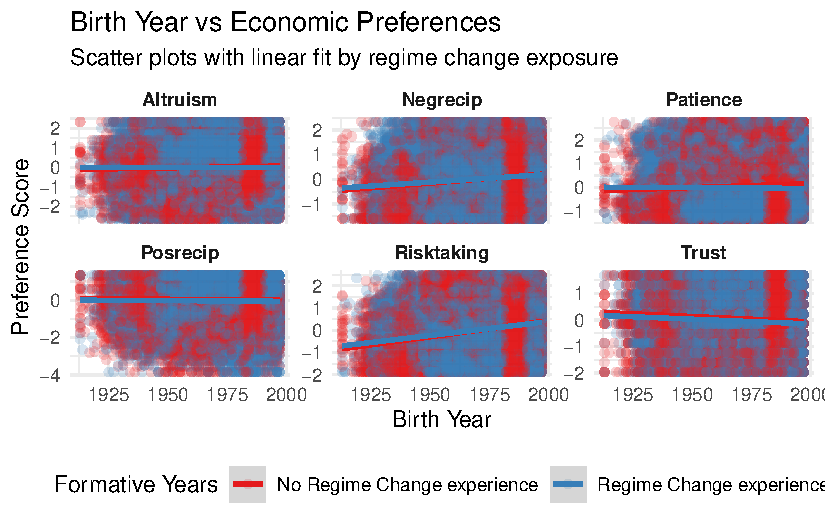
\includegraphics{Milestone-2-Data_files/figure-pdf/unnamed-chunk-9-2.pdf}

}

\end{figure}

\begin{Shaded}
\begin{Highlighting}[]
\CommentTok{\# Histograms}
\FunctionTok{print}\NormalTok{(histograms\_combined)}
\end{Highlighting}
\end{Shaded}

\begin{verbatim}
Warning: The dot-dot notation (`..density..`) was deprecated in ggplot2 3.4.0.
i Please use `after_stat(density)` instead.
\end{verbatim}

\begin{figure}[H]

{\centering \includegraphics{Milestone-2-Data_files/figure-pdf/unnamed-chunk-9-3.pdf}

}

\end{figure}

\begin{Shaded}
\begin{Highlighting}[]
\CommentTok{\# DiD plots}
\FunctionTok{print}\NormalTok{(did\_trust\_plot)}
\end{Highlighting}
\end{Shaded}

\begin{figure}[H]

{\centering \includegraphics{Milestone-2-Data_files/figure-pdf/unnamed-chunk-9-4.pdf}

}

\end{figure}

\begin{Shaded}
\begin{Highlighting}[]
\FunctionTok{print}\NormalTok{(did\_multi\_plot)}
\end{Highlighting}
\end{Shaded}

\begin{figure}[H]

{\centering \includegraphics{Milestone-2-Data_files/figure-pdf/unnamed-chunk-9-5.pdf}

}

\end{figure}

The following figures present additional visualizations of our data.

\begin{Shaded}
\begin{Highlighting}[]
\NormalTok{democracy\_2012 }\OtherTok{\textless{}{-}}\NormalTok{ vdem\_sub }\SpecialCharTok{\%\textgreater{}\%}
  \FunctionTok{filter}\NormalTok{(year }\SpecialCharTok{==} \DecValTok{2012}\NormalTok{) }\SpecialCharTok{\%\textgreater{}\%}
  \FunctionTok{select}\NormalTok{(country\_name,country\_text\_id, v2x\_libdem)}

\NormalTok{plot\_data }\OtherTok{\textless{}{-}} \FunctionTok{left\_join}\NormalTok{(country\_trust, democracy\_2012, }\AttributeTok{by =}\FunctionTok{c}\NormalTok{ (}\StringTok{"isocode"}\OtherTok{=} \StringTok{"country\_text\_id"}\NormalTok{))}


\FunctionTok{ggplot}\NormalTok{(final\_data\_gdp, }\FunctionTok{aes}\NormalTok{(}\AttributeTok{x =}\NormalTok{ age, }\AttributeTok{y =}\NormalTok{ trust, }\AttributeTok{color =}\NormalTok{ formative\_regime\_change)) }\SpecialCharTok{+} 
  \FunctionTok{geom\_smooth}\NormalTok{(}\AttributeTok{method =} \StringTok{"loess"}\NormalTok{, }\AttributeTok{se =} \ConstantTok{FALSE}\NormalTok{, }\AttributeTok{size =} \FloatTok{1.2}\NormalTok{) }\SpecialCharTok{+}
  \FunctionTok{theme\_minimal}\NormalTok{() }\SpecialCharTok{+}
  \FunctionTok{labs}\NormalTok{(}\AttributeTok{title =} \StringTok{"Trust Score by Age and Regime Change Exposure"}\NormalTok{,}
       \AttributeTok{x =} \StringTok{"Age"}\NormalTok{,}
       \AttributeTok{y =} \StringTok{"Trust Score"}\NormalTok{,}
       \AttributeTok{color =} \StringTok{"Formative Regime Change"}\NormalTok{)}
\end{Highlighting}
\end{Shaded}

\begin{verbatim}
`geom_smooth()` using formula = 'y ~ x'
\end{verbatim}

\begin{figure}[H]

{\centering \includegraphics{Milestone-2-Data_files/figure-pdf/unnamed-chunk-10-1.pdf}

}

\end{figure}

\begin{Shaded}
\begin{Highlighting}[]
\CommentTok{\# Merge democracy index into the individual{-}level dataset}
\NormalTok{mixed\_plot\_data }\OtherTok{\textless{}{-}} \FunctionTok{left\_join}\NormalTok{(final\_data\_gdp, democracy\_2012, }\AttributeTok{by =}\FunctionTok{c}\NormalTok{ (}\StringTok{"country"}\OtherTok{=} \StringTok{"country\_name"}\NormalTok{))}



\FunctionTok{ggplot}\NormalTok{(mixed\_plot\_data, }\FunctionTok{aes}\NormalTok{(}\AttributeTok{x =}\NormalTok{ subj\_math\_skills, }\AttributeTok{y =}\NormalTok{ trust, }\AttributeTok{color =}\NormalTok{ formative\_regime\_change)) }\SpecialCharTok{+} 
  \FunctionTok{geom\_smooth}\NormalTok{(}\AttributeTok{method =} \StringTok{"loess"}\NormalTok{, }\AttributeTok{se =} \ConstantTok{FALSE}\NormalTok{, }\AttributeTok{size =} \FloatTok{1.2}\NormalTok{) }\SpecialCharTok{+}
  \FunctionTok{theme\_minimal}\NormalTok{() }\SpecialCharTok{+}
  \FunctionTok{labs}\NormalTok{(}\AttributeTok{title =} \StringTok{"Trust Score vs. Subjective Math Skills by Regime Change Exposure"}\NormalTok{,}
       \AttributeTok{x =} \StringTok{"Subjective Math Skills"}\NormalTok{,}
       \AttributeTok{y =} \StringTok{"Trust"}\NormalTok{,}
       \AttributeTok{color =} \StringTok{"Formative Regime Change"}\NormalTok{)}
\end{Highlighting}
\end{Shaded}

\begin{verbatim}
`geom_smooth()` using formula = 'y ~ x'
\end{verbatim}

\begin{figure}[H]

{\centering \includegraphics{Milestone-2-Data_files/figure-pdf/unnamed-chunk-11-1.pdf}

}

\end{figure}

\hypertarget{refs}{}
\begin{CSLReferences}{1}{0}
\leavevmode\vadjust pre{\hypertarget{ref-coppedge_v-dem_2025}{}}%
Coppedge, Michael, John Gerring, Carl Henrik Knutsen, Staffan I.
Lindberg, Jan Teorell, David Altman, Fabio Angiolillo, et al. 2025.
{``V-Dem Dataset V15.''} Varieties of Democracy (V-Dem) Project.
\url{https://doi.org/10.23696/VDEMDS25}.

\leavevmode\vadjust pre{\hypertarget{ref-falk_global_2018}{}}%
Falk, Armin, Anke Becker, Thomas Dohmen, Benjamin Enke, David Huffman,
and Uwe Sunde. 2018. {``Global Evidence on Economic Preferences.''}
\emph{The Quarterly Journal of Economics} 133 (4): 1645--92.
\url{https://doi.org/10.1093/qje/qjy013}.

\end{CSLReferences}



\end{document}
